%------------------------------------------------------------------------------------------------------------------------
\chapter{モジュール量産におけるデータベースシステム}
\label{sec:chap6}
%------------------------------------------------------------------------------------------------------------------------

前章に示したように、次世代モジュールの量産の時にデータを適切に管理するためにデータベースシステムを開発している。

%測定と結果の一貫性と比較可能性を確保することが重要になる。
本章ではデータベースシステムの全体像について説明する。

%\begin{lstlisting}[caption=hoge,label=fuga, language=C++]
%#include<stdio.h>
%int main(){
%   printf("Hello world!");
%}
%\end{lstlisting}

%------------------------------------------------------------------------------------------------------------------------
\section{量産に用いるデータベースの概要}
\label{sec:DBforMasspro}
%------------------------------------------------------------------------------------------------------------------------

量産に用いるデータベースは、ITkの製造に関する情報を全てを記録するために開発されている中央データベースと、各研究機関でモジュール量産を管理するためのローカルデータベースがある。中央データベースとローカルデータベースの設置位置を\fref{fig:sekainohate}に示す。
本節ではそれぞれについての概要を示す。
\begin{figure}[tbp]
  \centering
  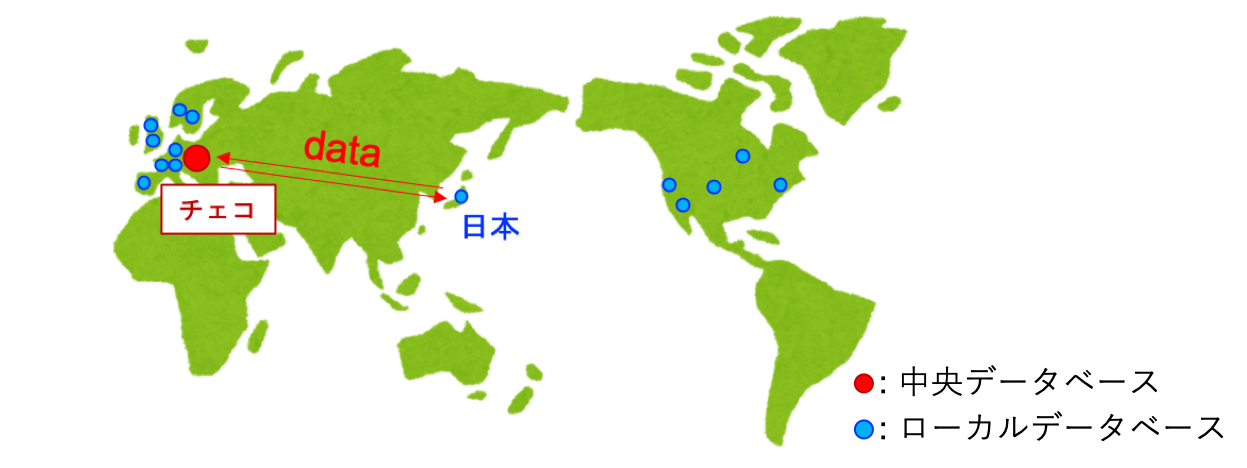
\includegraphics[height=5.5cm,keepaspectratio]{sekainohate.png}
  \caption[中央データベースとローカルデータベースの設置位置]{中央データベースとローカルデータベースの設置位置。ローカルデータベースは全てのモジュール組み立て機関に設置される。}
  \label{fig:sekainohate}
\end{figure}
%\begin{figure}[tbp]
%  \centering
%  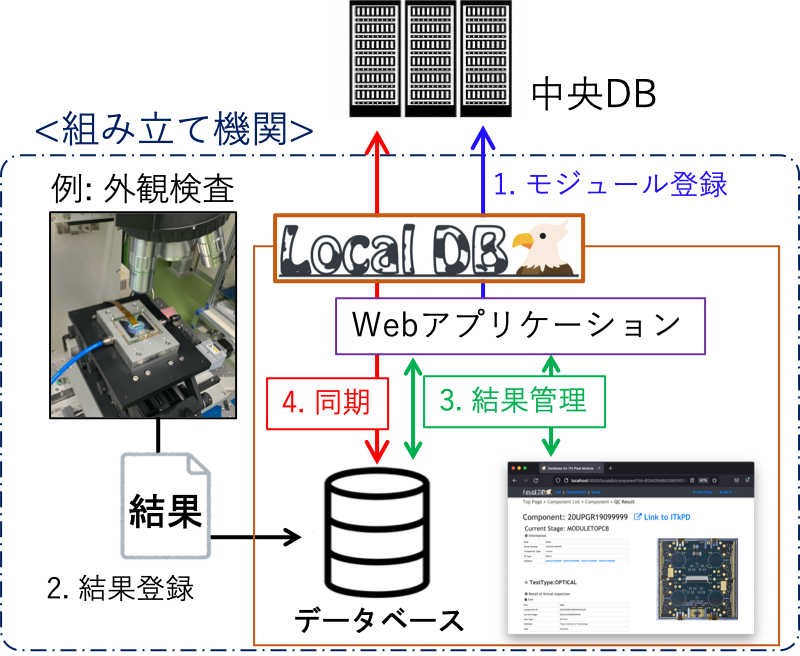
\includegraphics[height=7cm,keepaspectratio]{ryousanDB.png}
%  \caption[中央データベースとローカルデータベース]{中央データベースとローカルデータベース}
%  \label{fig:ryousanDB}
%\end{figure}

%------------------------------------------------------------------------------------------------------------------------
\subsection{中央データベース}
\label{sec:ITkPD}
%------------------------------------------------------------------------------------------------------------------------

中央データベースはITkに実装するためのピクセルモジュール・ストリップ検出器の量産についてのデータを管理することを目的として開発されている。ユニコーン大学が中心に開発を行っており、チェコにデータベースサーバーが設置されている。

ITkに実装される検出器とその構成部品は$50$万個程度であり、中央データベースではそれら全ての量産についてのデータを管理する。量産の組み立て工程で行われる試験結果は全てを記録するのではなく、ある品質管理試験における良い結果を一つのみを保存しておく。

中央データベースに保存されたデータは、ITkに配置するピクセルモジュールの選別に用いられる。$|\eta|$が小さい領域は通過する粒子の密度が高くなることが想定されるため、高い放射線量が予想される。そのため、ITkに搭載する際にはなるべく品質の良いモジュールを搭載する予定である。また、品質の悪いモジュールを配置する領域が固まると、その領域を通過する飛跡の再構成が難しくなり、物理解析の際に不良データと判別されてしまうことがある。そこで、品質の悪いモジュールの領域が固まらないように配置する必要
がある。この選別に用いる参考値として、中央データベースに保存されているデータを用いる予定である。

また、運転前後で検出器に損傷が起きていないかを確認するためにもこれらの値を用いる。運転前後の読み出し試験やその他の試験の結果の比較を行うことにより、センサーへの放射線損傷や不良ピクセルの推移等を確認することができる。
ITkは約$10$年間の運転が予定されており、少なくとも$20$年間は検出器についてのデータが利用できるようにしておく予定である。



%------------------------------------------------------------------------------------------------------------------------
\subsection{ローカルデータベース}
\label{sec:LocalDB}
%------------------------------------------------------------------------------------------------------------------------

ローカルデータベースは各研究機関に設置され、モジュールの組み立て工程における品質試験結果を管理するためのシステムである。ローカルデータベースは各研究機関におけるモジュールの品質試験結果を全て記録しておくという点で中央データベースとは異なる。

先述したように、モジュールの組み立て工程およびそれぞれの工程の際に行われる品質試験の数は非常に多く、それぞれのモジュールに対して適切に試験を管理する必要がある。モジュールの量産は各研究機関において$\mathcal{O}(100)\sim \mathcal{O}(1000)$個であり、1つのモジュールについて$30$項目程度の品質試験を行うため、$\mathcal{O}(10000)$個の試験結果を適切に管理する必要がある。各組み立て機関において、適切にデータを管理し、かつピクセルモジュールの量産を円滑に行うことができるようにサポートするために\textbf{ローカルデータベース}というシステムを開発している。ローカルデータベースに対する要求は以下のようなものである。
\begin{itemize}
  \item 検出器情報や試験結果の情報を他研究機関との整合性を保ちつつ管理すること。
  \item ピクセルモジュールの量産を円滑に行うことができるようサポートすること。
  \item 中央のデータベースにモジュール量産に関わるデータを同期すること。
\end{itemize}

以上の目標を達成するために、東工大を中心にローカルデータベースの開発が進められている。次節において、ローカルデータベースの構造と、先行研究における開発項目について示す。

%------------------------------------------------------------------------------------------------------------------------
\section{ローカルデータベースの構造}
\label{sec:AboutLocalDB}
%------------------------------------------------------------------------------------------------------------------------
ローカルデータベースの構造の全体像を\fref{fig:localdbsystem}に示す。ローカルデータベースは品質試験結果を保有しておくためのデータベースであるMongoDBと、データベースに保存されたデータを操作および閲覧するためのウェブアプリケーションから構成される。MongoDBへの試験結果の登録は、読み出し試験については専用のソフトウェアであるYARRを用いて行い、それ以外の品質試験については大阪大学および都立大学によって開発が進められている品質試験結果登録用GUIを用いて行う。
本節では、MongoDBとウェブアプリケーションについて説明する。


\begin{figure}[tbp]
  \centering
  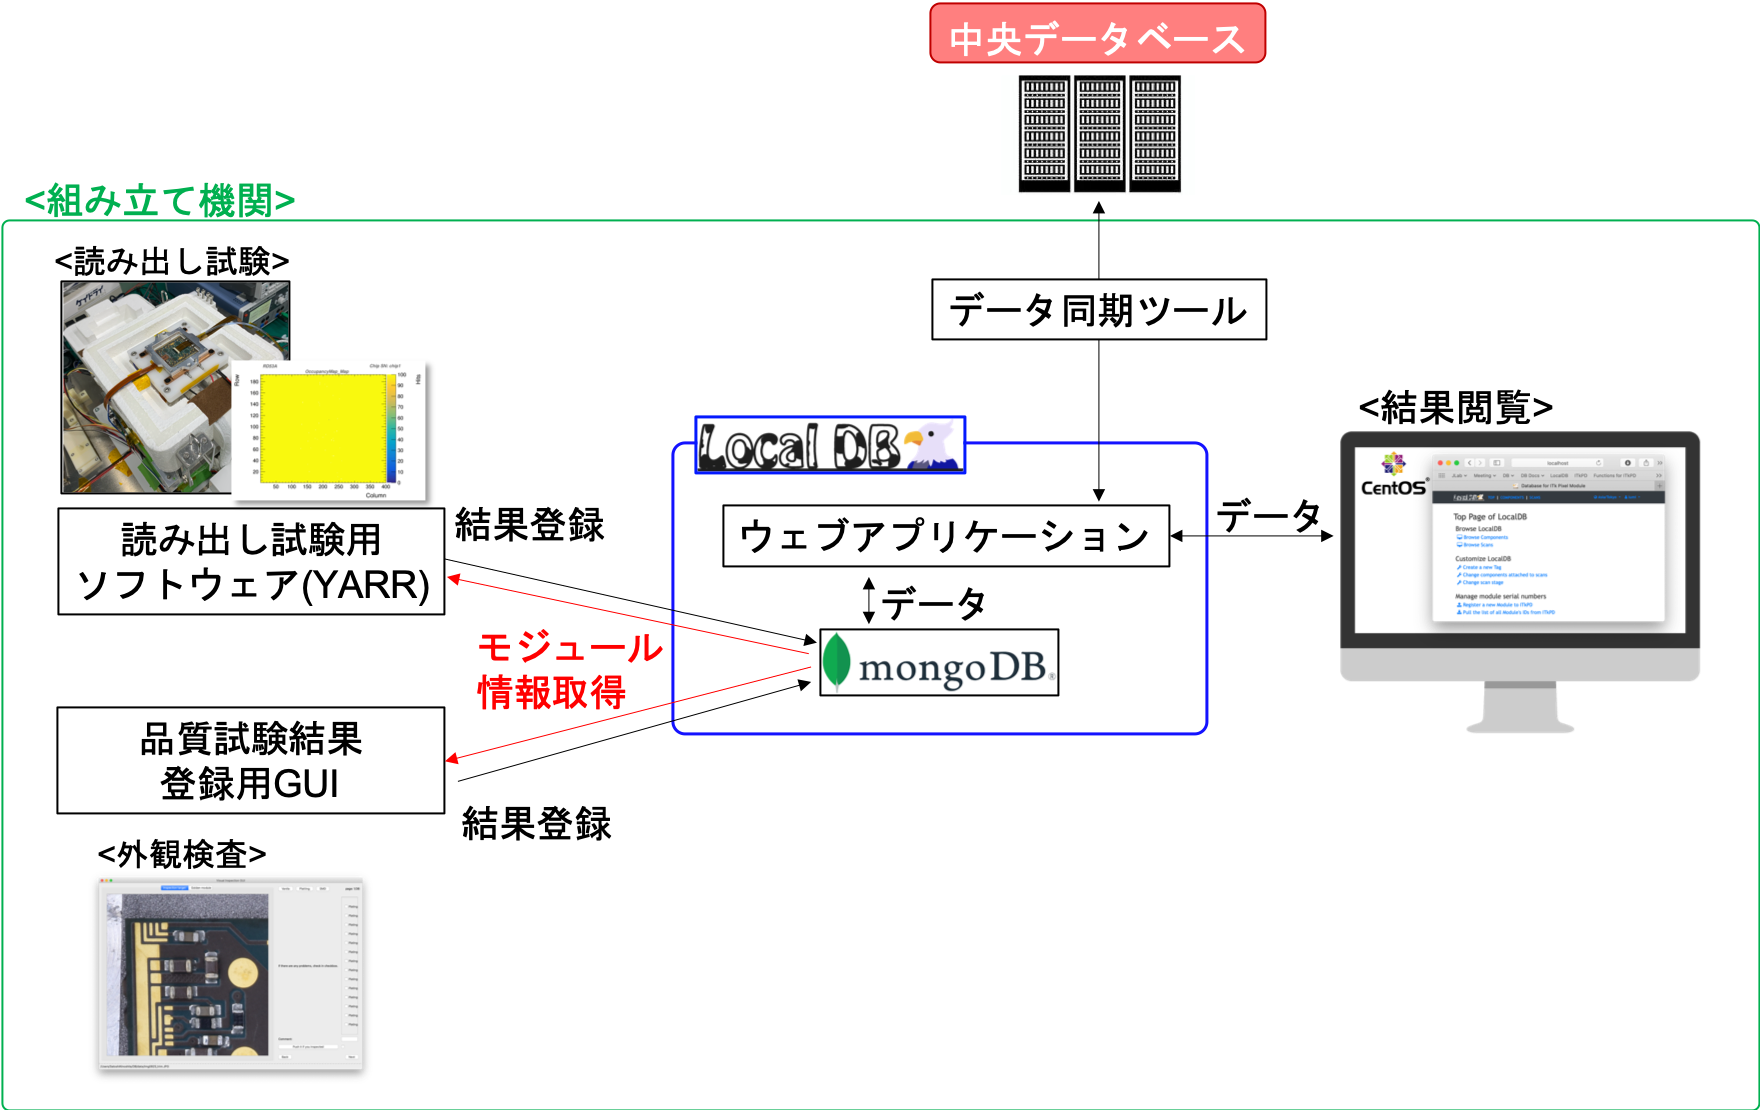
\includegraphics[height=7cm,keepaspectratio]{localdbsystem.png}
  \caption[ローカルデータベースの全体像]{ローカルデータベースの全体像。ローカルデータベースはMongoDBとウェブアプリケーションから構成され、品質試験結果を管理するための複合的な機能を持つ。}
  \label{fig:localdbsystem}
\end{figure}

%------------------------------------------------------------------------------------------------------------------------
\subsection{MongoDB\cite{mongo}}
\label{sec:mongo}
%------------------------------------------------------------------------------------------------------------------------

MongoDBはアプリケーションの開発や拡張を簡単に行うことができるように設計されている、オープンソースのドキュメントデータベースである。ドキュメントデータベースは、非リレーショナルデータベース(NoSQL)の一種であり、1つのデータをドキュメントと呼び、具体的にはデータをJSON\footnote{JSONとは\textbf{J}ava\textbf{S}cript \textbf{O}bject \textbf{N}otation の略で、データ記述言語の一種である。あるkeyとvalueを対応させることにより、データを取り出すことができる。ウェブアプリケーションでデータを転送する場合に使われることが多い。}のようなドキュメントとして保存する。MongoDBでは、\textbf{BSON}という、JSONに非常によく似た形式のデータを扱い、binary表記したデータを持つためJSONよりも多くのデータの型を保存することができる。

MongoDBでは、データベース、コレクション、ドキュメント(オブジェクト)の概念を用いてデータを管理する。各ドキュメントはコレクションという枠の中に格納され、さらに各コレクションはデータベースによって包括される。
各コレクション間の関係を自由に定義することができ、データベースが構造化し、階層的な性質を持たせてデータを管理することができる。
%\fref{fig:mongoimage}にMongoDBのデータを保管するための概念図を示す。

%\begin{figure}[tbp]
%  \centering
%  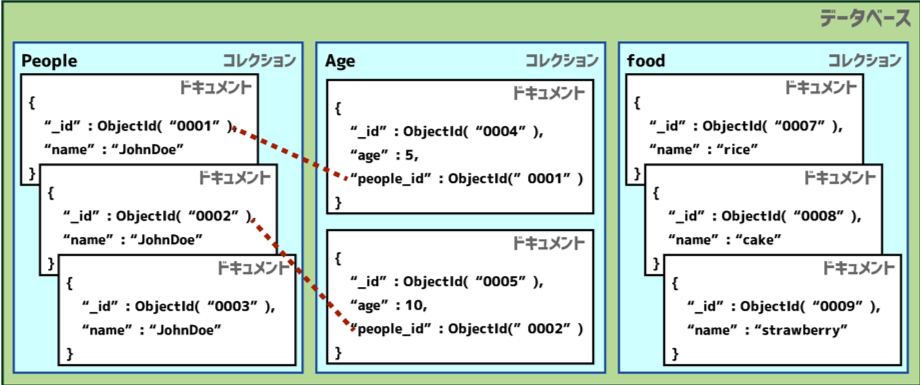
\includegraphics[height=7cm,keepaspectratio]{mongoimage.png}
%  \caption[MongoDBの全体像]{MongoDBの全体像}
%  \label{fig:localdb-collection}
%\end{figure}

各ドキュメントは\textbf{オブジェクトID}という$12\ \si{bite}$のIDによって管理される。オブジェクトIDはデータ生成時の時間情報によって決まる値($4\ \si{bite}$)、データベースマシンによってランダムに生成される値($5\ \si{bite}$)、データベースマシンのカウンターによって生成される値($3\ \si{bite}$)により自動生成される。そのため、複数のドキュメントが同一のオブジェクトIDを持つことはなく、これにより識別を行うことができる。また、オブジェクトIDを用いることにより、異なるコレクションにおけるドキュメント間の関連付けを行い、データベース内の構造を柔軟に設計することができる。

\begin{lstlisting}[caption=MongoDBのドキュメントの例,label=mongodocument, language=Python]
{
  {
    "_id": ObjectId("6038c960b9a87924947df638"),
    "year": 2015,
    "title": "The Big New Movie",
    "info": {
      "plot": "Nothing happens at all.",
      "rating": 0
    }
  }
}
\end{lstlisting}


ローカルデータベースシステムの開発において、MongoDBを使う利点を以下に示す。
\begin{itemize}
  \item スキーマレスで、ドキュメント構造を動的に変更することができる。 \\
  品質管理試験は、試験項目により保存するパラメータが異なる。格納形式に柔軟性のあるNoSQLのMongoDBを用いることにより、同一コレクションに異なる形式の試験結果を保管しておくことができる。また、現在は試作器を用いて、次世代器の品質試験に向けた実験装置の準備や試験のレビューを行っている。そのため、最終的にデータベースに残る結果が変わることがある。この際、NoSQLのMongoDBでは変更点が最小に抑えることができるので、開発スピードを早くできることが多い。
%  \item JSON形式でデータを保持するため整形が容易である。\\
%  We love JSON format.
  \item ObjectIdにより、中央データベースとの整合性を保ちやすい。 \\
  中央データベースで管理するデータは$12\ \si{byte}$のIDを保持している。そのため、中央データベースにおけるIDとローカルデータベースのMongoDBにおけるObjectIdを関連付けて管理することが可能になる。
\end{itemize}

%%------------------------------------------------------------------------------------------------------------------------
%\subsection{LocalDBのデータ管理構造}
%\label{sec:localDB-structure}
%%------------------------------------------------------------------------------------------------------------------------
これらの利点から、MongoDBを用いてローカルデータベースの開発を行っている。ローカルデータベースにおけるモジュール情報および品質管理に用いるコレクションを\tref{tab:local-collection}に示す。ローカルデータベースにおいて、\textbf{localdb}と\textbf{localdbtool}の2つのデータベースを準備している。localdbはピクセルモジュール情報および品質管理試験結果等の各組み立て機関から中央データベースに共有する情報を保有し、localdbtoolはユーザー情報、中央データベースからダウンロードした組み立て機関のリストやピクセルモジュールの構成要素等の中央データベースに共有しない情報や組み立て機関に依存しない情報を保有する。
各コレクション間の関係を\fref{fig:localdb-collection}に示す。このように各コレクションに保存する情報を関連付けて管理することにより、品質試験結果やそれに関する情報をデータベースから取り出しやすくなる。

\begin{table}[tbp]
  \begin{center}
    \caption[ローカルデータベースのコレクション]{ローカルデータベースのコレクション一覧。}
    \label{tab:local-collection}
    \begin{tabular}{|l||l|l|}
    \hline
      データベース名 & コレクション名 & 保存情報 \\
    \bhline{1.5pt}
      \multirow{11}{*}{localdb}
       & component & モジュール情報、FE チップ情報 \\
       & childParentRelation & FE チップとモジュールの関係性 \\
       & testRun & 読み出し試験結果 \\
       & componentTestRun & component と testRun の関係性 \\
       & user & 読み出し試験実施者 \\
       & institute & 読み出し試験実施場所 \\
       & comments & 部品、試験結果についてのコメント情報 \\
       & QC.module.status & 各モジュールに対する組み立て工程及び選択された試験結果 \\
       & QC.result & 品質試験結果 \\
       & QC.prop.status & ワイヤー配線の後に決まるモジュール特性の書き換え情報 \\
       & QC.module.prop & モジュール特性の情報 \\
    \hline
      \multirow{5}{*}{localdbtools}
       & QC.status & 組み立て工程及び試験項目 \\
       & QC.module.types & モジュールの構成部品 \\
       & viewer.user & ローカルデータベースのユーザ情報 \\
       & viewer.query & 読み出し結果キーワード、検索機能実行時に使用 \\
       & viewer.tag.docs & モジュールや試験結果に付けるタグの情報 \\
    \hline
    \end{tabular}
  \end{center}
\end{table}

\begin{figure}[tbp]
  \centering
  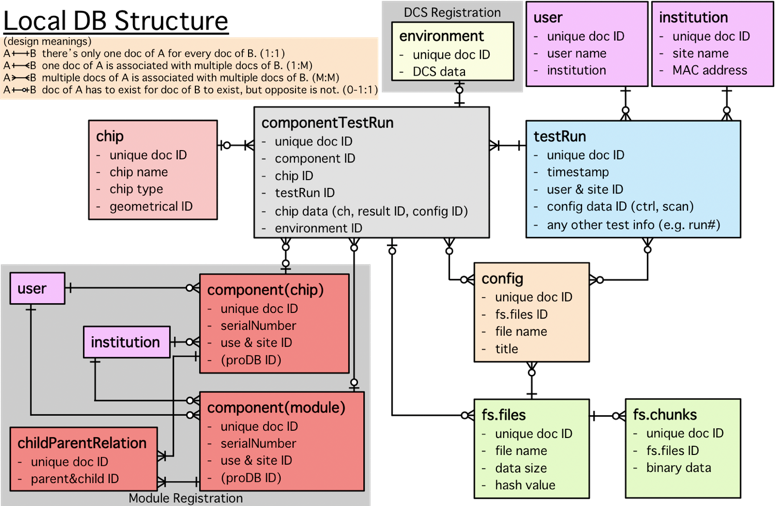
\includegraphics[height=13cm,keepaspectratio]{localdbcollection.png}
  \caption[ローカルデータベースの構造]{ローカルデータベースの構造。それぞれの四角はコレクションを表しており、緑色は使用ユーザーに関する情報、赤色は部品についての情報、青色はYARRを用いて登録した読み出し試験結果、紫は品質試験結果登録用GUIを用いて登録した結果についてのものである。また、灰色はモジュールの組み立て工程を管理するためのコレクションであり、黄色は読み出し試験データや画像データを管理するファイルシステムに関するコレクションである。直線はオブジェクトIDによるドキュメント間の関連付けを表しており、直線が十字になっている場合は1つのドキュメントとの関連付け、分岐しているものは複数本のドキュメントと関連付け、丸印は関連付けされていない可能性があることを表している。}
  \label{fig:localdb-collection}
\end{figure}



%------------------------------------------------------------------------------------------------------------------------
\subsection{ウェブアプリケーション}
\label{sec:flask}
%------------------------------------------------------------------------------------------------------------------------

各研究機関において、ローカルデータベースを使用するために、試験者がデータベースに保存されている品質試験結果を閲覧および管理を簡単にできる必要がある。
しかし、MongoDBはデータ構造が柔軟であり、使用用途に基づき多様なデータベース構造が考えられるため、データベース内のデータを表示・処理するインターフェースは提供されておらず、必要に応じて適宜インターフェースを開発する必要がある。
ローカルデータベースシステムでは、多様な利用者がデータベース内のデータを閲覧、操作を実現できることを目標として、PythonのウェブアプリケーションフレームワークであるFlaskを導入している。

ウェブアプリケーションの処理を\fref{fig:webapp}に示す。利用者が見るウェブブラウザのインターフェイスはhtmlで書き、ボタンを押したらPythonのバックエンド側にパラメータが送信される。受信したパラメータをもとにFlaskで処理を返し、html側で表示を行う。Flaskが受け取った処理を行う際、MongoDBに保存するデータを操作するために、PythonのパッケージであるPyMongoを用いている。また、ウェブブラウザにおいて、動的な処理を行う際にはJavaScriptを利用している。この流れにより、ウェブブラウザから、データベースに保存されているデータを簡単に取り扱うことができるように設計している。

\begin{figure}[tbp]
  \centering
  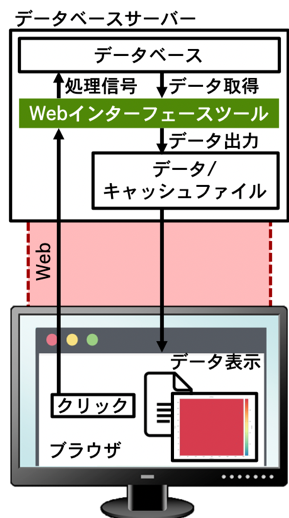
\includegraphics[height=4cm,keepaspectratio]{localdbwebapp.png}
  \caption[ウェブアプリケーションの処理の概念図]{ウェブアプリケーションの処理の概念図。図中の数字は処理の順序を表し、ウェブブラウザから送信した信号に基づきウェブアプリケーション内で処理を行う。}
  \label{fig:webapp}
\end{figure}
%\begin{figure}[tbp]
%  \centering
%  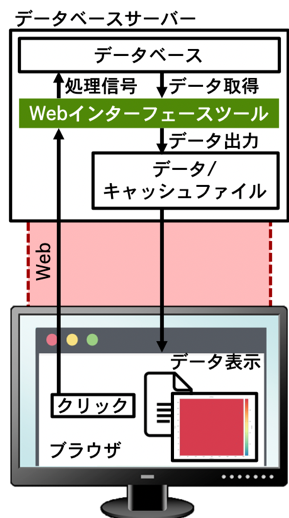
\includegraphics[height=7cm,keepaspectratio]{localdbwebapp.png}
%  \caption[ローカルデータベースシステムの全体像]{ローカルデータベースシステムの全体像}
%  \label{fig:webbrowser}
%\end{figure}

%------------------------------------------------------------------------------------------------------------------------
\section{モジュールの品質試験に必要な開発項目}
\label{sec:okubottan}
%------------------------------------------------------------------------------------------------------------------------

東工大を中心に開発が進められており、これまでは読み出し試験を中心に開発が進められている。モジュールの品質管理に必要な開発項目および開発状況を以下に示す。
\begin{itemize}
  \item[1.] データベース構造の設計 \\
  \fref{fig:localdb-collection}に示したように、MongoDBにおけるコレクションを定義し、データを取り出しやすく工夫している。読み出し試験についてのデータベース構造は先行研究\cite{kubotan,kimu}によって定義され、非読み出し試験およびモジュールの組み立て工程を管理するためのデータベース構造は先行研究\cite{oku}を行った奥山氏と私が開発を行った。
  \item[2.] 試験結果管理機能
  \begin{itemize}
    \item[2-1.] 読み出し試験 \\
    読み出し試験の結果の閲覧および解析機能は先行研究\cite{oku,kubotan}によって開発が行われた。読み出し試験はピクセルの読み出し性能の不良判定するのに重要な試験であり、各組み立て工程で品質に変化がないこと、あるいは不良ピクセルが発生した際にどの工程で問題があったかを発見することが重要である。本研究では、各組み立て工程間で評価できる機能を追加した。これについて\ref{sec:hyouji}に示す。
    \item[2-2.] 非読み出し試験 \\
    非読み出し試験の閲覧機能はこれまで未開発であり、本研究においてこの機能を実装した。閲覧機能について、\ref{sec:hyouji}に示す。
  \end{itemize}
  \item[3.] モジュール組み立て工程管理機能 \\
  各組み立て機関で$\mathcal{O}(100)$〜$\mathcal{O}(1000)$個のモジュールを量産するため、それぞれのモジュールについて品質試験が適切に行われたこと、各工程で全ての結果が揃っていることを担保する必要がある。この機能は先行研究\cite{oku}によって開発が行われたが、モジュール特性の結果管理についてまだ未開発であった。これについて\ref{sec:kanri}に示す。
  \item[4.] 中央データベースとの同期機能 \\
  これまで、モジュールを中央データベースからダウンロードする機能、および読み出し試験の結果を中央データベースと同期する機能の開発が先行研究\cite{oku}によって行われてきた。しかし、モジュールを中央データベースへ登録、非読み出し試験の結果およびモジュールの組み立て工程を中央データベースと同期する機能については未開発であった。これについて、\ref{sec:upload-result}に示す。
\end{itemize}






\newpage
